\chapter{긴 끈과 블랙홀의 대응}

\lectureoverview{블랙홀에는 엔트로피가 있으므로 미시적 자유도를 가져야 한다. 여기서는 그 자유도를 끈 이론으로 설명하는 가장 단순한 방법을 구성한다. 먼저 들뜬 긴 끈의 상태 수를 세고, 이어서 끈과 블랙홀의 기술이 만나는 지점까지 끈 결합을 바꾼다. 마지막 등식은 다음 강의에서 완성할 문제로 일부러 남겨 둔다.}

\section{엔트로피가 요구하는 미시적 구성 요소}

어떤 계의 엔트로피가 크다는 것은 그 계가 많은 양의 미시적 정보를 감출 수 있다는 뜻이다. 뜨거운 물이 담긴 욕조의 엔트로피는 \(10^{30}\) 정도일 수 있다. 물 분자를 하나씩 살펴보든 그렇지 않든, 이 사실만으로도 미시적 자유도가 어마어마하게 많다는 것을 알 수 있다. 열역학은 에너지와 온도를 측정해 엔트로피를 결정할 수 있지만, 그 엔트로피를 지닌 대상이 무엇인지는 밝혀 주지 않는다.

유체역학을 보면 이 구분이 익숙하게 다가온다. 유체역학은 원자를 언급하지 않고 밀도, 속도, 압력, 거시적 흐름을 기술한다. 여기에 열역학을 더하면 유체에 엔트로피가 있다는 사실을 알게 된다. 엔트로피는 거친 눈금으로 기술한 방정식에는 드러나지 않는 미시적 구조가 있음을 알린다. 이는 답을 주기보다 새로운 질문을 던진다.

블랙홀은 같은 문제를 더 선명하게 제기한다. 베켄슈타인의 제안에 호킹의 계산이 더해져, 블랙홀의 엔트로피는 사건의 지평선 면적에 비례한다고 알려져 있다. 일반 상대성 이론은 기하와 열역학을 결정하지만 미시적 상태의 목록을 제공하지는 않는다. 면적 법칙을 설명하는 수많은 작은 대상은 무엇이며, 그 배치는 어떠한가? 끈 이론에는 구체적인 후보가 있다. 여기서 전개할 논증은 의도적으로 정성적이다. 수치 상수와 완전한 상태 수 계산의 형식적 도구는 생략하면서도 매개변수 의존성은 올바르게 구한다.

\section{세 가지 척도와 표기상의 주의점}

중력에는 특별한 길이 척도인 플랑크 길이가 있다.
\begin{equation}
\ell_p=\sqrt{\frac{G_N\hbar}{c^3}}.
\label{eq:l06-planck-si}
\end{equation}

\begin{classroomqa}
\audiencequestion{\(G_N\), \(\hbar\), \(c\)의 어떤 조합이 플랑크 길이를 주나요?\lecturetimestamp{00:06:08}}
\lecturerresponse{그 값은 \(\sqrt{G_N\hbar/c^3}\)이며, 대략 \(10^{-33}\) 센티미터입니다. 곧바로 \(\hbar=c=1\)로 두면 관계식이 훨씬 간단해집니다.}
\end{classroomqa}

자연 단위계에서는
\begin{equation}
\hbar=c=1,
\qquad
G_N=\ell_p^2.
\label{eq:l06-planck-area}
\end{equation}
따라서 뉴턴 상수의 차원은 면적이다. 그러므로 면적을 \(G_N\)로 나누면 무차원량이 되어 엔트로피가 될 수 있다.

끈 이론에는 두 번째 길이인 \(\ell_s\)가 있다. 끈을 가열하거나 높은 들뜬 상태에 두면 여러 척도에서 진동한다. 이 기본적인 그림에서 특징적인 최소 척도는 끈 길이다. \(\ell_s\)를 끈 진동의 기본 단위 하나에 해당하는 크기로 볼 수 있다.

세 번째 양은 무차원 끈 결합 \(g_s\)이다. 이는 끈의 분리와 결합을 제어한다. 끈이 두 끈으로 갈라지거나 들뜬 끈이 닫힌 끈 양자를 방출할 수 있다.

\begin{classroomqa}
\audiencequestion{끈 결합의 물리적 의미는 무엇인가요?\lecturetimestamp{00:09:20}}
\lecturerresponse{끈이 자기 자신과 교차할 때 갈라지는 경우처럼, 끈 상호작용이 일어날 가능성을 제어합니다. 더 정확히 말하면 \(g_s\)는 상호작용 진폭이고, 이에 대응하는 확률이나 붕괴율은 \(g_s^2\) 차수부터 나타납니다.}
\end{classroomqa}

방출되는 질량 없는 닫힌 끈 들뜸은 중력자일 수 있다. 그런 점에서 \(g_s\)는 전하와 비슷한 역할을 한다. 상호작용 꼭짓점에 붙는 인자이기 때문이다.\editorialnote{강의에서는 \(g_s\)를 확률이라고도 하고 진폭이라고도 한다. 섭동론에서 이는 진폭 수준의 결합이며, 확률과 붕괴율에는 그 제곱이 들어간다.}

\section{중력이 \texorpdfstring{\(g_s^2\)}{결합의 제곱을 아는 이유}}

먼저 전자기학에서 교환 그림을 생각해 보자. 전하를 띤 한 물체가 \(e\)의 인자를 가진 광자를 방출하고, 다른 물체가 \(e\)의 인자를 가지고 그 광자를 흡수한다. 따라서 교환 진폭에는 \(e^2\)가 들어간다. 이 그림은 고전적인 발사체가 실제로 날아가는 상황을 뜻하지는 않지만, 결합이 어떻게 들어가는지는 정확히 보여 준다.

\begin{figure}[htbp]
\centering
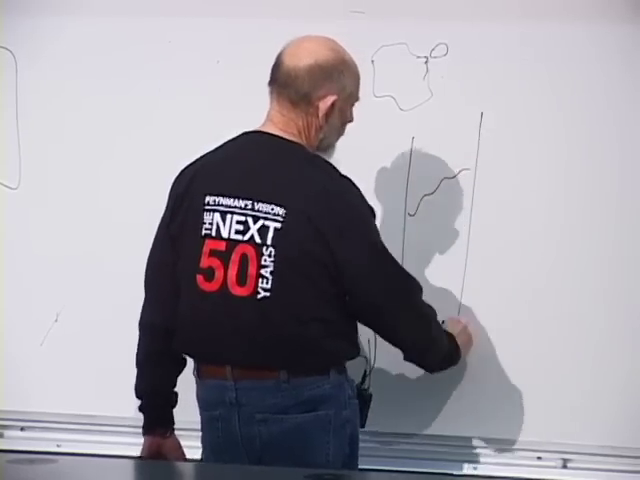
\includegraphics[width=0.72\textwidth]{lecture_06_figure_03.png}
\caption{칠판에 완성된 교환 그림. 방출과 흡수에 각각 결합 인자가 붙어 있다.}
\lectureframe{00:11:30.000}
\end{figure}

끈 이론에서는 광자가 중력자로, 전하가 \(g_s\)로 바뀐다. 방출에 하나, 흡수에 하나씩 인자가 붙으므로 중력의 세기는 \(g_s^2\)에 비례한다.

먼 거리에 있는 같은 상호작용은 뉴턴의 힘 법칙을 재현해야 한다.
\begin{equation}
F_{\mathrm{grav}}\sim G_N\frac{M_1M_2}{r^2}.
\end{equation}
질량과 역제곱 의존성은 원천과 전파를 나타낸다. 여기서 필요한 점은 그 항들에 곱해지는 결합이다.

\begin{figure}[htbp]
\centering
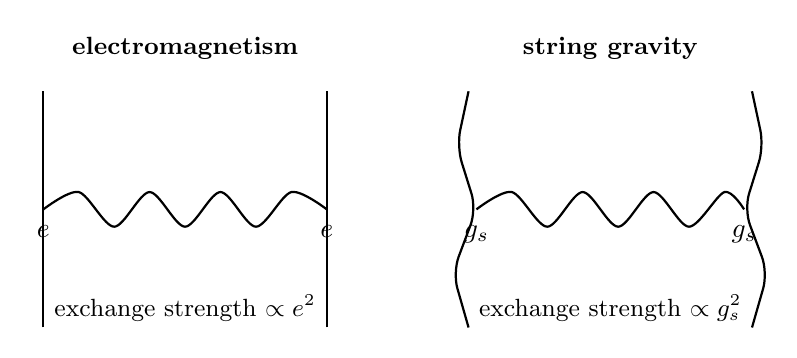
\begin{tikzpicture}[x=1cm,y=1cm]
  \node[font=\small\bfseries] at (1.8,3.55) {electromagnetism};
  \draw[line width=0.8pt] (0,0) -- (0,3);
  \draw[line width=0.8pt] (3.6,0) -- (3.6,3);
  \draw[line width=0.8pt] plot[smooth] coordinates {(0,1.5) (0.45,1.72) (0.9,1.28) (1.35,1.72) (1.8,1.28) (2.25,1.72) (2.7,1.28) (3.15,1.72) (3.6,1.5)};
  \node[below] at (0,1.42) {\(e\)};
  \node[below] at (3.6,1.42) {\(e\)};
  \node[font=\small] at (1.8,0.25) {exchange strength \(\propto e^2\)};
  \node[font=\small\bfseries] at (7.2,3.55) {string gravity};
  \draw[line width=0.8pt,rounded corners=6pt] (5.4,0) -- (5.2,0.7) -- (5.5,1.5) -- (5.25,2.3) -- (5.4,3);
  \draw[line width=0.8pt,rounded corners=6pt] (9,0) -- (9.2,0.7) -- (8.9,1.5) -- (9.15,2.3) -- (9,3);
  \draw[line width=0.8pt] plot[smooth] coordinates {(5.5,1.5) (5.95,1.72) (6.4,1.28) (6.85,1.72) (7.3,1.28) (7.75,1.72) (8.2,1.28) (8.65,1.72) (8.9,1.5)};
  \node[below] at (5.5,1.42) {\(g_s\)};
  \node[below] at (8.9,1.42) {\(g_s\)};
  \node[font=\small] at (7.2,0.25) {exchange strength \(\propto g_s^2\)};
\end{tikzpicture}
\caption{결합을 세는 비유. 교환되는 양자의 양 끝에서 각각 하나의 상호작용 인자가 기여한다.}
\end{figure}

이 관찰로 뉴턴 상수를 거의 결정할 수 있다. 결합 \(g_s\)는 무차원인 반면, 4차원에서 \(G_N\)의 차원은 길이의 제곱이다. 쓸 수 있는 미시적 길이는 \(\ell_s\)이므로,
\begin{equation}
G_N\sim g_s^2\ell_s^2.
\label{eq:l06-newton-string}
\end{equation}
이를 식~\eqref{eq:l06-planck-area}과 결합하면 다음을 얻는다.
\begin{equation}
\ell_p\sim g_s\ell_s.
\label{eq:l06-planck-string}
\end{equation}

\begin{figure}[htbp]
\centering
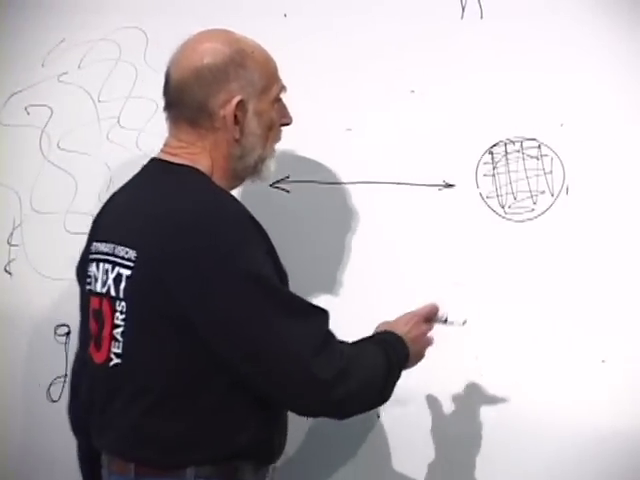
\includegraphics[width=0.72\textwidth]{lecture_06_figure_04.png}
\caption{칠판에 남겨 둔 기본 관계식: \(\ell_p^2=G_N\)와 \(\ell_p\sim g_s\ell_s\).}
\lectureframe{00:15:45.000}
\end{figure}

식~\eqref{eq:l06-newton-string}은 이 강의 전반에서 사용하는 단순화된 관계식이다.\editorialnote{콤팩트화된 끈 이론에서 유효한 4차원 뉴턴 상수는 콤팩트화 부피와 1 정도 크기의 관례에도 의존한다. 강의에서는 대응 관계의 스케일링에 초점을 맞추기 위해 그 정보를 생략한다.}

\begin{classroomqa}
\audiencequestion{\(g_s\)은 1보다 큰가요, 작은가요? 또 어느 길이가 더 큰가요?\lecturetimestamp{00:16:00}}
\lecturerresponse{결합이 약한 영역인 \(g_s<1\)에서 다룹니다. 그러면 \(\ell_p\sim g_s\ell_s\)에 따라 끈 길이가 플랑크 길이보다 큽니다. 강결합에서는 다른 기술이 필요하지만, 여기서는 다루지 않아도 됩니다.}
\end{classroomqa}

\section{블랙홀의 상태 수}

볼츠만 상수와 수치 인자를 생략하면 베켄슈타인--호킹 엔트로피는 다음과 같다.
\begin{equation}
S_{\mathrm{BH}}=\frac{A}{4G_N}sim\frac{A}{G_N}sim\frac{A}{\ell_p^2}.
\label{eq:l06-bh-area}
\end{equation}
반고전적 공식에서 \(1/4\) 인자는 정확한 값이지만, 이 스케일링 논증에서는 아무 역할도 하지 않는다.

\begin{classroomqa}
\audiencequestion{아래 첨자 ``BH''는 블랙홀을 뜻하나요, 베켄슈타인--호킹을 뜻하나요?\lecturetimestamp{00:16:51}}
\lecturerresponse{우리에게는 둘 다 떠올리게 하는 표기로 보면 됩니다. 핵심은 엔트로피가 플랑크 면적 단위로 잰 사건의 지평선 면적이라는 점입니다.}
\end{classroomqa}

4차원 슈바르츠실트 블랙홀의 경우,
\begin{equation}
R_s=2G_NM,
\qquad
A=4\pi R_s^2.
\end{equation}
강의에서처럼 \(2\)와 \(4\pi\)를 생략하면,
\begin{align}
S_{\mathrm{BH}}
&\sim \frac{R_s^2}{G_N}
\sim \frac{(G_NM)^2}{G_N} \\
&\sim M^2G_N
\sim M^2\ell_p^2.
\label{eq:l06-bh-mass}
\end{align}
이 형태를 끈의 상태 수와 비교할 것이다.

\section{랜덤 워크로 보는 긴 끈}

작은 끈에서 시작해 에너지를 주입하자. 일반적인 고도로 들뜬 끈은 단정한 고리 모양으로 남아 있지 않는다. 감긴 낚싯줄을 잘못 풀었을 때처럼 길고 복잡하게 얽힌 물체가 된다. 거시적으로는 서로 구별되지 않는 배치가 매우 많기 때문에 이 얽힌 끈에는 엔트로피가 있다.

상태 수를 세기 위해 공간을 링크의 길이가 \(\ell_s\)인 격자로 바꿔 생각하자. 꼭짓점은 격자점이고 선은 링크이며, 기본 정사각형은 면이다. 끈은 연결된 링크들의 연속으로 나타낸다. 이 모형은 의도적으로 거칠게 단순화했지만, 상태 수의 지수적 증가는 원하는 스케일링을 포착한다.

\begin{figure}[htbp]
\centering
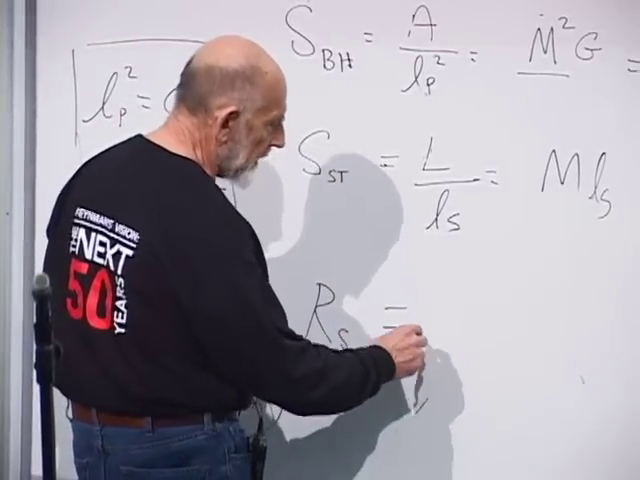
\includegraphics[width=0.72\textwidth]{lecture_06_figure_05.png}
\caption{2차원 격자 모형. 파란 선분은 끈의 한 걸음을 나타내며, 각 격자점에서 가능한 네 가지 다음 경로를 센다.}
\lectureframe{00:23:50.000}
\end{figure}

\begin{classroomqa}
\audiencequestion{이 단순한 워크에서는 매 단계마다 몇 가지 선택지가 있나요?\lecturetimestamp{00:22:43}}
\lecturerresponse{제곱 격자에서는 네 가지입니다. 바로 되돌아가는 경로도 허용하기 때문입니다. 3차원에서는 여섯 가지가 됩니다. 다른 격자를 쓰면 보통의 수는 달라지지만, 링크 수가 늘어남에 따라 워크 수가 지수적으로 증가한다는 점은 변하지 않습니다.}
\end{classroomqa}

끈에 \(n\)개의 링크가 있으면, 2차원 단순 모형에서 상태 수는 다음과 같다.
\begin{equation}
\Omega_n\sim4^n.
\label{eq:l06-walk-count}
\end{equation}
예외적으로 곧게 뻗은 워크 하나가 있지만, 이는 \(4^n\)개 상태 가운데 하나에 불과하다. 전형적인 워크는 여러 차례 접히며 얽힌 덩어리를 이룬다. \(n\)가 크면 무작위로 만든 거의 모든 배치는 질적으로 서로 비슷해 보인다.

거시적으로 구별할 수 없는 배치의 수에 로그를 취하면 엔트로피가 된다.
\begin{equation}
S_{\mathrm{st}}=\log\Omega_n\sim n\log4\sim n.
\label{eq:l06-string-entropy-n}
\end{equation}

\begin{classroomqa}
\audiencequestion{왜 엔트로피는 \(4^n\)이 아니라 \(n\)에 비례하게 되나요?\lecturetimestamp{00:25:39}}
\lecturerresponse{엔트로피는 상태 수의 로그입니다. 따라서 \(\log(4^n)=n\log4\)이고, 인자 \(\log4\)은 1 정도의 상수이므로 생략하겠습니다.}
\end{classroomqa}

끈의 한쪽 끝에서 다른 쪽 끝까지 따라가며 잰 윤곽 길이가 \(L\)라면,
\begin{equation}
n=\frac{L}{\ell_s},
\qquad
S_{\mathrm{st}}\sim\frac{L}{\ell_s}.
\label{eq:l06-string-entropy-length}
\end{equation}
여기서 \(L\)는 얽힌 덩어리의 지름이 아니다. 끈을 따라 잰 훨씬 더 긴 거리다.

이제 윤곽 길이를 질량으로 바꾸자. \(c=\hbar=1\)에서는 질량의 차원이 길이의 역수다. 따라서 끈 길이 하나에 해당하는 링크 하나의 질량은 대략
\begin{equation}
m_{\mathrm{link}}\sim\frac{1}{\ell_s}.
\label{eq:l06-link-mass}
\end{equation}

\begin{classroomqa}
\audiencequestion{링크 하나의 질량이 왜 \(1/\ell_s\)에 비례해야 하나요?\lecturetimestamp{00:29:20}}
\lecturerresponse{이 단위계에서 질량은 길이의 역수이고, 쓸 수 있는 유일한 길이는 \(\ell_s\)입니다. 달리 말해, \(1/\ell_s^2\) 정도의 끈 장력에 링크 길이 \(\ell_s\)를 곱해도 같은 결과를 얻습니다.}
\end{classroomqa}

그러면 끈 전체의 질량은
\begin{equation}
M\sim n m_{\mathrm{link}}
\sim\frac{n}{\ell_s}
\sim\frac{L}{\ell_s^2},
\qquad
L\sim M\ell_s^2.
\label{eq:l06-string-mass}
\end{equation}
식~\eqref{eq:l06-string-entropy-length}에 대입하면 다음을 얻는다.
\begin{equation}
S_{\mathrm{st}}\sim M\ell_s.
\label{eq:l06-string-entropy-mass}
\end{equation}
격자 워크는 월드시트 제약 조건과 수치 계수를 무시하지만, 고도로 들뜬 끈 스펙트럼의 지수적 증가는 이와 같은 선도 스케일링을 준다.\editorialnote{랜덤 워크 구성은 끈 상태의 높은 준위 밀도를 기억하기 위한 도식일 뿐, 기본 끈을 실제로 이산화한 것은 아니다.}

\section{논증의 출발점이 되는 불일치}

이제 두 결과를 나란히 놓으면 다음과 같다.
\begin{equation}
S_{\mathrm{BH}}\sim M^2\ell_p^2,
\qquad
S_{\mathrm{st}}\sim M\ell_s.
\label{eq:l06-two-entropies}
\end{equation}
두 식은 서로 비슷해 보이지만, 질량을 고정하고 결합을 임의로 택하면 같지 않다. 블랙홀 식은 \(M\)의 제곱에 비례하고, 끈 식은 선형으로 비례한다. 뜨거운 끈을 아무 설명 없이 블랙홀이라고 선언할 수는 없다. 두 영역이 어떻게 이어지는지 밝혀야 한다.

\begin{figure}[htbp]
\centering
\includegraphics[width=0.78\textwidth]{lecture_06_figure_06.png}
\caption{가림 없이 칠판에 나란히 적은 비교: 위에는 블랙홀 엔트로피, 아래에는 긴 끈 엔트로피가 있고, 왼쪽에는 플랑크--끈 관계식이 남아 있다.}
\lectureframe{00:33:20.000}
\end{figure}

여기서 강의는 잠시 멈춘다. 긴장감을 남기는 것은 유익하다. 이 불일치는 발상이 틀렸다는 뜻이 아니라, 중력의 세기를 바꾸면서 동일한 상태를 비교해야 한다는 단서다.

\section{결합의 조절 손잡이를 돌리기}

\(\ell_s\)를 고정하고 \(g_s\)를 바꿀 수 있다고 생각해 보자. \(g_s=0\)에서는 끈이 분리되거나 결합하지 않으며, \(G_N\sim g_s^2\ell_s^2\)이므로 중력도 사라진다. 따라서 에너지가 충분히 큰 상태는 길고 상호작용이 약한 끈이다.

\(g_s\)를 천천히 키우자. 끈 상호작용이 가능해지고, 지금 논증에서 더 중요한 것은 중력이 강해진다는 점이다.

\begin{classroomqa}
\audiencequestion{\(g_s\)를 키우면, 가장 먼저 끈이 짧은 끈들로 갈라지기만 하나요?\lecturetimestamp{00:36:29}}
\lecturerresponse{분리와 결합이 가능해지지만, \(\ell_s\)를 고정하고 엔트로피가 높은 상태를 따라가 봅시다. 핵심 효과는 \(G_N\)가 커져 긴 끈의 자기중력이 얽힌 덩어리를 안쪽으로 끌어당기는 것입니다.}
\end{classroomqa}

물체는 수축하며 밀도가 높아진다. 중력 퍼텐셜 에너지는 음수이므로, 수축하면 총에너지가 낮아지고 따라서 질량도 감소한다.

\begin{classroomqa}
\audiencequestion{자기중력이 끈을 끌어당길 때 에너지는 증가하나요, 감소하나요?\lecturetimestamp{00:37:48}}
\lecturerresponse{감소합니다. 결합 에너지는 더 음수가 됩니다. 같은 상태를 계속 따라가더라도 그 경로를 따라 질량이 일정할 필요는 없습니다.}
\end{classroomqa}

결국 물체의 크기는 슈바르츠실트 반지름과 비슷해진다. 그 지점을 지나면 블랙홀로 기술하는 것이 자연스럽다. 초기 들뜸이 클수록 더 작은 결합에서 이 조건에 도달한다. 질량이 큰 물체일수록 사건의 지평선을 만들기 위해 필요한 중력의 세기가 더 약하기 때문이다.

\begin{figure}[htbp]
\centering
\resizebox{0.95\linewidth}{!}{%
\begin{tikzpicture}[x=1cm,y=1cm,>=Latex]
  \draw[->,line width=0.9pt] (0,0) -- (11,0) node[right] {increasing \(g_s\)};
  \node[draw,rounded corners,align=center,minimum width=2.6cm,minimum height=1.15cm] at (1.8,1.5) {long excited string\\weak self-gravity};
  \node[draw,rounded corners,align=center,minimum width=2.6cm,minimum height=1.15cm] at (5.5,1.5) {correspondence point\\\(R_s\sim\ell_s\)};
  \node[draw,circle,align=center,minimum size=1.8cm] at (9.3,1.5) {black\\hole};
  \draw[->,line width=0.8pt] (3.15,1.5) -- (4.1,1.5) node[midway,above,font=\small] {contracts};
  \draw[->,line width=0.8pt] (6.9,1.5) -- (8.25,1.5);
  \node[font=\small,align=center] at (5.5,-0.65) {same family of states followed slowly;\\binding energy and mass may change};
\end{tikzpicture}
}
\caption{\(\ell_s\)를 고정한 대응 경로. 화살표를 거꾸로 따라가면 블랙홀 상태가 긴 끈 상태로 돌아간다.}
\end{figure}

\begin{classroomqa}
\audiencequestion{\(g_s\)가 0과 1 사이에 있다고 생각하면 되나요?\lecturetimestamp{00:40:18}}
\lecturerresponse{그렇습니다. 논증은 약결합 영역에서 이루어집니다. \(g_s\)가 매우 작으면 상태가 블랙홀이 되려면 그에 맞게 질량이 커야 합니다. 제어가 어려운 \(g_s>1\) 영역에 들어갈 필요는 없습니다.}
\end{classroomqa}

이 사고실험에서 느린 변화는 가역적이다.

\begin{classroomqa}
\audiencequestion{중력이 블랙홀을 붙들어 두지 못할 때까지 결합을 다시 낮추면, 블랙홀은 무엇이 되나요?\lecturetimestamp{00:41:37}}
\lecturerresponse{긴 끈이 됩니다. 이 구성에서 중력이 사라지면 모든 것은 끈 상태로 기술되어야 합니다. 조절 손잡이를 한쪽으로 돌리면 끈이 블랙홀이 되고, 반대로 돌리면 블랙홀이 끈이 됩니다.}
\end{classroomqa}

총에너지와 부피를 고정하면, 엔트로피가 가장 큰 배치는 짧은 끈이 엄청나게 많은 상태라기보다 사실상 긴 끈 하나다. 이 명제는 여기서 유도하지 않는다. 하게도 영역에 가까운 끈의 통계역학에서 나오는 결과이며, 뒤에서 다시 다룬다.

\section{외부 관찰자가 보는 것}

물체가 블랙홀로 기술될 때 끈은 어디에 있는가? 외부 관찰자의 기술에서는 끈이 갑자기 사라지지 않는다. 슈바르츠실트 시간으로 보면 겉보기에는 사건의 지평선을 통과하는 시각이 무한히 늦어지므로, 끈의 자유도는 지평선 위나 그 근처에 쌓이는 것으로 나타난다.

\begin{figure}[htbp]
\centering
\includegraphics[width=0.72\textwidth]{lecture_06_figure_07.png}
\caption{거시적 지평선에서는 끈 길이 척도의 구조가 얇은 흐림층처럼 보이는 반면, 반지름이 고리 척도에 가까운 작은 지평선에서는 그 구조가 어떻게 보이는지 칠판에 비교해 그렸다.}
\lectureframe{00:45:30.000}
\end{figure}

\(R_s\gg\ell_s\)일 때 블랙홀은 거시적이며, 지평선 반지름에 비하면 끈 길이 척도의 구조는 얇은 층에 불과하다. 반지름이 \(\ell_s\)에 가까워지면 매끄러운 블랙홀과 늘어난 끈의 구분은 의미를 잃는다. 이것은 외부 관찰자의 늘어난 지평선 기술이다. 낙하하는 물질이 정칙한 지평선을 결코 통과하지 않는다는 좌표 독립적 주장과 혼동해서는 안 된다.\editorialnote{강의에서는 블랙홀 상보성에서 익숙한 외부 영역의 기술을 사용한다. 지평선``위''라는 표현은 외부 관찰자의 기술로 분해해 볼 수 있는 자유도를 가리키며, 그 자유도의 공변적인 위치를 따로 유도했다는 뜻은 아니다.}

전이는 다음 조건에서 일어난다.
\begin{equation}
R_s\sim\ell_s.
\label{eq:l06-correspondence-radius}
\end{equation}
끈 척도보다 작은 영역에서는 슈바르츠실트 기하가 블랙홀을 지탱한다고 여겨지는 구조를 분해해 볼 수 없다. 고리들은 예상되는 지평선에서 벗어나 요동하므로, 그 상태는 끈이라고 부르는 편이 더 적절하다.

\section{대응점}

식~\eqref{eq:l06-correspondence-radius}에 \(R_s\sim G_NM\)를 사용하면,
\begin{equation}
G_NM\sim\ell_s.
\end{equation}
그다음 \(G_N\sim g_s^2\ell_s^2\)를 대입하면,
\begin{equation}
M g_s^2\ell_s^2\sim\ell_s,
\qquad
M g_s^2\ell_s\sim1.
\label{eq:l06-correspondence-condition}
\end{equation}

\begin{figure}[htbp]
\centering
\includegraphics[width=0.72\textwidth]{lecture_06_figure_08.png}
\caption{칠판에 완성한 전이 계산: \(R_s\sim\ell_s\)에서 상자 안의 무차원 조건 \(Mg_s^2\ell_s\sim1\)을 얻는다.}
\lectureframe{00:49:50.000}
\end{figure}

청중 가운데 한 사람이 이 조건이 무엇을 예고하는지 알아차렸다. 대응점에서는
\begin{align}
S_{\mathrm{BH}}
&\sim M^2\ell_p^2
\sim M^2g_s^2\ell_s^2 \\
&=(M\ell_s)(Mg_s^2\ell_s)
\sim M\ell_s
\sim S_{\mathrm{st}}.
\label{eq:l06-entropy-preview}
\end{align}

\begin{classroomqa}
\audiencequestion{이 방정식들은 블랙홀 엔트로피와 끈 엔트로피가 같아짐을 이미 함의하나요?\lecturetimestamp{00:50:18}}
\lecturerresponse{그렇습니다. 계산이 바로 그 결론으로 향하고 있습니다. 필요한 재료는 칠판에 나와 있지만, 대응 관계의 논리를 차근차근 다시 살펴볼 수 있도록 강의에서는 이 재료들을 완전히 결합하는 일을 뒤로 미룹니다.}
\end{classroomqa}

식~\eqref{eq:l06-entropy-preview}은 문답에서 암묵적으로 예고된 한 줄짜리 대수 계산이다. 이는 스케일링을 확립하지만 정확한 계수 \(1/4\)까지 정하지는 않는다. 정확한 미시적 일치를 얻으려면 더 통제 가능한 블랙홀과 더 상세한 끈 구성이 필요하다.\editorialnote{강의는 식~\eqref{eq:l06-entropy-preview}을 완성된 유도로 제시하기 전에 끝난다. 청중이 등식을 분명히 짚었고 필요한 관계식이 모두 앞서 나왔으므로, 여기에는 식을 명시해 두었다.}

\section{엔트로피를 보존할 수 있는 이유}

마지막으로 논리적 요소 하나가 남아 있다. 계가 고립되어 있고 변화가 가역적일 때, 자기장이나 \(g_s\) 같은 제어 매개변수를 충분히 천천히 바꾼다고 하자. 에너지, 크기, 결합 에너지는 달라질 수 있지만 엔트로피는 보존된다.
\begin{equation}
\Delta S=0.
\label{eq:l06-adiabatic-entropy}
\end{equation}
강의에서는 이를 정보 보존과 연결한다. 엔트로피는 거친 눈금의 기술에 가려진 정보를 측정한다. 해밀토니안을 천천히 가역적으로 바꾸면 그 정보는 없어지지 않고 상태들이 재배열된다.

\begin{classroomqa}
\audiencequestion{엔트로피를 일정하게 유지하려면 경로가 상전이를 피해야 하나요?\lecturetimestamp{00:54:01}}
\lecturerresponse{그렇습니다. 상태를 연속적으로 따라갈 수 있어야 합니다. 유한한 계에는 무한 부피계와 같은 의미에서 비해석적인 열역학적 상전이가 엄밀히 존재하지 않습니다. 변화가 충분히 느리면 대응 관계를 매끄러운 교차로 다룰 수 있습니다.}
\end{classroomqa}

여기서 단열은 더 강한 의미인 준정적이고 가역적인 과정으로 사용된다. 단열이더라도 비가역 과정에서는 엔트로피가 생성될 수 있다. 느린 변화와 상태를 추적할 수 있다는 점이 핵심이다.\editorialnote{열역학적 명제 \(\Delta S=0\)에는 가역 단열 경로가 필요하다. 양자역학적으로 이에 대응하는 생각은 매개변수가 변하는 동안 제어되지 않은 준위 전이가 일어나지 않게 하면서 동일한 상태 집합을 따라가는 것이다.}

\begin{classroomqa}
\audiencequestion{같은 총질량을 지닌 짧은 끈 여러 개보다 긴 끈 하나의 엔트로피가 더 큰 이유는 무엇인가요?\lecturetimestamp{00:54:44}}
\lecturerresponse{직관에 어긋나지만, 유한한 부피에서 고에너지 상태 수를 직접 세어 보면 긴 끈 성분이 우세합니다. 증명은 뒤로 미룬다. 지금 논증에 필요한 것은 블랙홀이 매우 많은 짧은 끈으로 이루어진 희박한 기체가 아니라 최대 엔트로피 끈 부문으로 대응한다는 점뿐이다.}
\end{classroomqa}

따라서 실제로 따를 전략은 다음과 같다.
\begin{enumerate}
\item \(M_0\)의 질량과 \(g_{s,0}\)의 결합을 가진 블랙홀에서 시작한다.
\item \(g_s\)를 천천히 낮추면서 엔트로피가 높은 동일한 상태 계열을 따라간다.
\item \(R_s\sim\ell_s\)에서 멈춘다. 이 지점에서는 블랙홀 기술이 긴 끈 기술로 바뀐다.
\item \(S_{\mathrm{st}}\sim M\ell_s\)를 사용해 끈 상태 수를 센다.
\item 그 엔트로피를 가역 경로를 따라 원래 블랙홀까지 보존한다.
\end{enumerate}

\begin{figure}[htbp]
\centering
\includegraphics[width=0.72\textwidth]{lecture_06_figure_09.png}
\caption{전략을 설명하는 동안 칠판에 남겨 둔 원리: \(g_s\)의 단열 변화는 \(S\)를 바꾸지 않는다.}
\lectureframe{00:56:40.000}
\end{figure}

끈 이론은 전하를 띠거나 회전하는 블랙홀, 초대칭 블랙홀, 극한에 가까운 블랙홀, 고차원 블랙홀의 엔트로피를 훨씬 정밀하게 셈해 왔다. 여기서 다룬 중성 슈바르츠실트 블랙홀은 거친 대응 논증으로, 상태 밀도의 매개변수 의존성과 물리적 교차를 밝힐 뿐 보호된 축퇴도의 정확한 값을 구하지는 않는다.\editorialnote{결합이 변해도 상태 수가 보호되는 특별한 블랙홀에서 정확한 일치가 가장 잘 성립한다. 이 강의에서는 의도적으로 가장 단순한 크기 정도의 계산을 제시한다.}

\begin{classroomqa}
\audiencequestion{중력을 끄면 상태가 끈 하나로 정확히 이루어지는 대신 끈 두 개로 이루어질 수도 있나요?\lecturetimestamp{00:58:25}}
\lecturerresponse{긴 끈이 소수만 존재할 확률은 유한하며, 끈 하나 대신 둘을 사용해도 엔트로피의 선도적 스케일링은 달라지지 않습니다. 논증을 바꾸게 될 것은 짧은 끈으로 이루어진 거대한 기체로의 분열이지만, 고에너지 통계적 계수는 그런 결과를 선호하지 않습니다.}
\end{classroomqa}

블랙홀은 한 영역 안에 담을 수 있는 엔트로피가 가장 큰 상태이며, 중력을 제거했을 때 이에 대응하는 고엔트로피 상태는 긴 끈이다. 이제 두 기술은 연결되었지만, 아직 정밀한 계산으로 발전하지는 않았다. 다음 단계에서는 대수 계산을 꼼꼼히 반복하고 이 대응 관계를 어디까지 신뢰할 수 있는지 살펴본다.
